% Created by tikzDevice version 0.7.0 on 2015-01-10 18:41:33
% !TEX encoding = UTF-8 Unicode
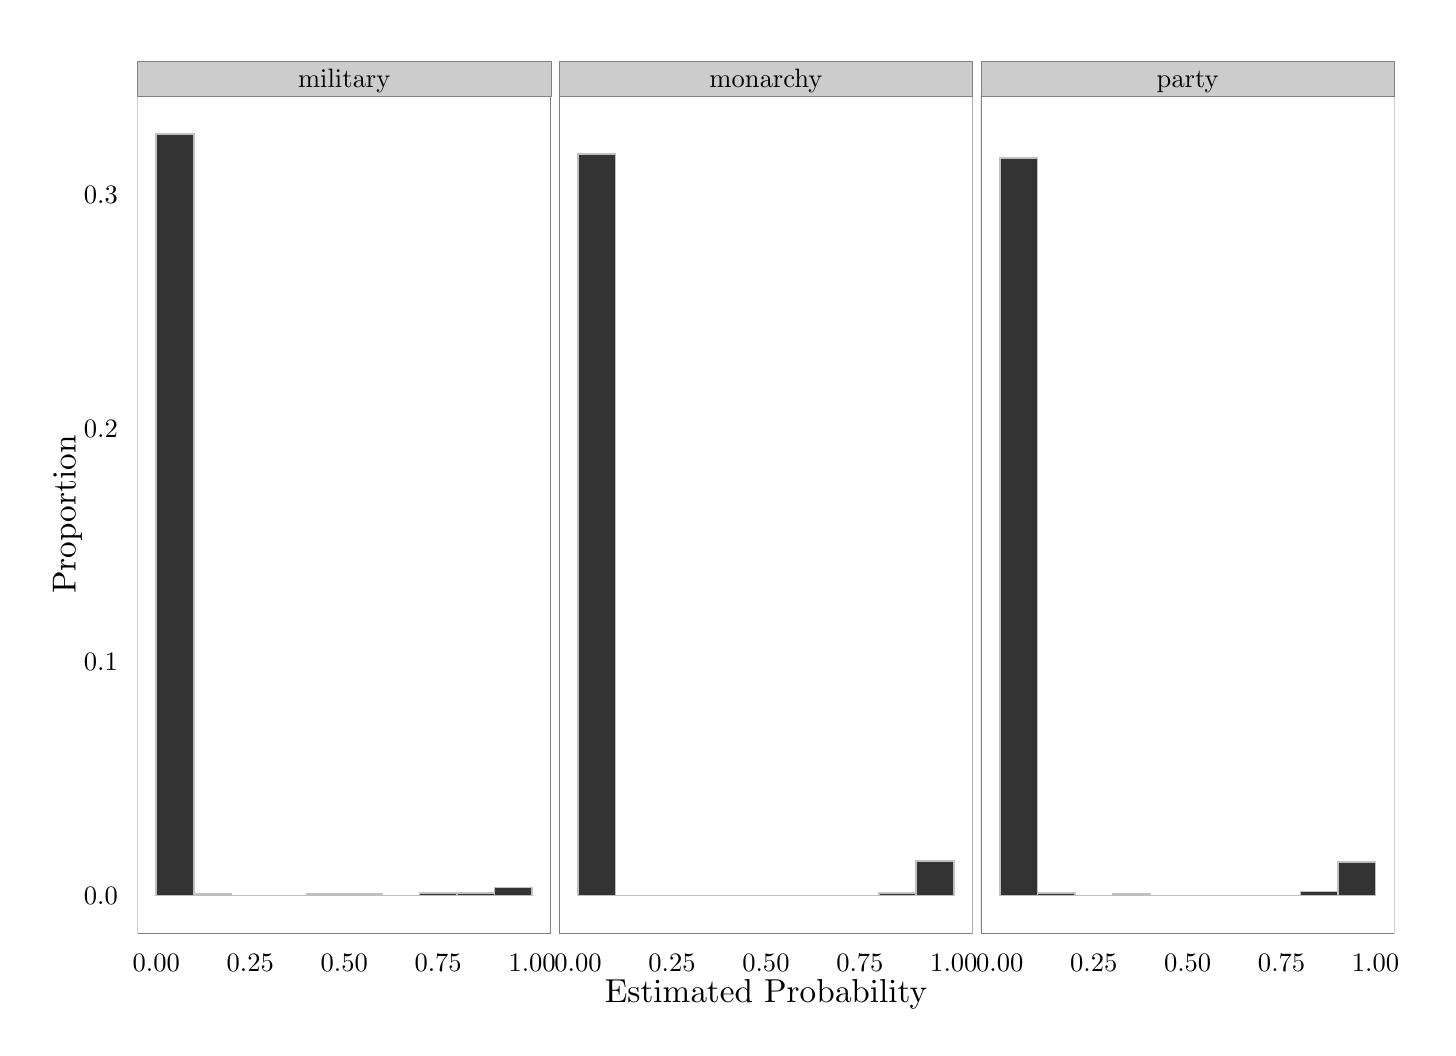
\begin{tikzpicture}[x=1pt,y=1pt]
\definecolor[named]{fillColor}{rgb}{1.00,1.00,1.00}
\path[use as bounding box,fill=fillColor,fill opacity=0.00] (0,0) rectangle (505.89,361.35);
\begin{scope}
\path[clip] (  0.00,  0.00) rectangle (505.89,361.35);
\definecolor[named]{drawColor}{rgb}{1.00,1.00,1.00}
\definecolor[named]{fillColor}{rgb}{1.00,1.00,1.00}

\path[draw=drawColor,line width= 0.6pt,line join=round,line cap=round,fill=fillColor] (  0.00,  0.00) rectangle (505.89,361.35);
\end{scope}
\begin{scope}
\path[clip] ( 39.69, 34.03) rectangle (189.07,336.67);
\definecolor[named]{fillColor}{rgb}{1.00,1.00,1.00}

\path[fill=fillColor] ( 39.69, 34.03) rectangle (189.07,336.67);
\definecolor[named]{drawColor}{rgb}{0.75,0.75,0.75}
\definecolor[named]{fillColor}{rgb}{0.20,0.20,0.20}

\path[draw=drawColor,line width= 0.6pt,line join=round,fill=fillColor] ( 46.48, 47.79) rectangle ( 60.06,322.91);

\path[draw=drawColor,line width= 0.6pt,line join=round,fill=fillColor] ( 60.06, 47.79) rectangle ( 73.64, 48.27);

\path[draw=drawColor,line width= 0.6pt,line join=round,fill=fillColor] ( 73.64, 47.79) rectangle ( 87.22, 47.79);

\path[draw=drawColor,line width= 0.6pt,line join=round,fill=fillColor] ( 87.22, 47.79) rectangle (100.80, 47.79);

\path[draw=drawColor,line width= 0.6pt,line join=round,fill=fillColor] (100.80, 47.79) rectangle (114.38, 48.27);

\path[draw=drawColor,line width= 0.6pt,line join=round,fill=fillColor] (114.38, 47.79) rectangle (127.96, 48.27);

\path[draw=drawColor,line width= 0.6pt,line join=round,fill=fillColor] (127.96, 47.79) rectangle (141.54, 47.79);

\path[draw=drawColor,line width= 0.6pt,line join=round,fill=fillColor] (141.54, 47.79) rectangle (155.12, 48.76);

\path[draw=drawColor,line width= 0.6pt,line join=round,fill=fillColor] (155.12, 47.79) rectangle (168.70, 48.76);

\path[draw=drawColor,line width= 0.6pt,line join=round,fill=fillColor] (168.70, 47.79) rectangle (182.28, 50.69);
\definecolor[named]{drawColor}{rgb}{0.50,0.50,0.50}

\path[draw=drawColor,line width= 0.6pt,line join=round,line cap=round] ( 39.69, 34.03) rectangle (189.07,336.67);
\end{scope}
\begin{scope}
\path[clip] (192.08, 34.03) rectangle (341.46,336.67);
\definecolor[named]{fillColor}{rgb}{1.00,1.00,1.00}

\path[fill=fillColor] (192.08, 34.03) rectangle (341.46,336.67);
\definecolor[named]{drawColor}{rgb}{0.75,0.75,0.75}
\definecolor[named]{fillColor}{rgb}{0.20,0.20,0.20}

\path[draw=drawColor,line width= 0.6pt,line join=round,fill=fillColor] (198.87, 47.79) rectangle (212.45,315.67);

\path[draw=drawColor,line width= 0.6pt,line join=round,fill=fillColor] (212.45, 47.79) rectangle (226.03, 47.79);

\path[draw=drawColor,line width= 0.6pt,line join=round,fill=fillColor] (226.03, 47.79) rectangle (239.61, 47.79);

\path[draw=drawColor,line width= 0.6pt,line join=round,fill=fillColor] (239.61, 47.79) rectangle (253.19, 47.79);

\path[draw=drawColor,line width= 0.6pt,line join=round,fill=fillColor] (253.19, 47.79) rectangle (266.77, 47.79);

\path[draw=drawColor,line width= 0.6pt,line join=round,fill=fillColor] (266.77, 47.79) rectangle (280.35, 47.79);

\path[draw=drawColor,line width= 0.6pt,line join=round,fill=fillColor] (280.35, 47.79) rectangle (293.93, 47.79);

\path[draw=drawColor,line width= 0.6pt,line join=round,fill=fillColor] (293.93, 47.79) rectangle (307.51, 47.79);

\path[draw=drawColor,line width= 0.6pt,line join=round,fill=fillColor] (307.51, 47.79) rectangle (321.09, 48.76);

\path[draw=drawColor,line width= 0.6pt,line join=round,fill=fillColor] (321.09, 47.79) rectangle (334.67, 60.34);
\definecolor[named]{drawColor}{rgb}{0.50,0.50,0.50}

\path[draw=drawColor,line width= 0.6pt,line join=round,line cap=round] (192.08, 34.03) rectangle (341.46,336.67);
\end{scope}
\begin{scope}
\path[clip] (344.47, 34.03) rectangle (493.85,336.67);
\definecolor[named]{fillColor}{rgb}{1.00,1.00,1.00}

\path[fill=fillColor] (344.47, 34.03) rectangle (493.85,336.67);
\definecolor[named]{drawColor}{rgb}{0.75,0.75,0.75}
\definecolor[named]{fillColor}{rgb}{0.20,0.20,0.20}

\path[draw=drawColor,line width= 0.6pt,line join=round,fill=fillColor] (351.26, 47.79) rectangle (364.84,314.23);

\path[draw=drawColor,line width= 0.6pt,line join=round,fill=fillColor] (364.84, 47.79) rectangle (378.42, 48.76);

\path[draw=drawColor,line width= 0.6pt,line join=round,fill=fillColor] (378.42, 47.79) rectangle (392.00, 47.79);

\path[draw=drawColor,line width= 0.6pt,line join=round,fill=fillColor] (392.00, 47.79) rectangle (405.58, 48.27);

\path[draw=drawColor,line width= 0.6pt,line join=round,fill=fillColor] (405.58, 47.79) rectangle (419.16, 47.79);

\path[draw=drawColor,line width= 0.6pt,line join=round,fill=fillColor] (419.16, 47.79) rectangle (432.74, 47.79);

\path[draw=drawColor,line width= 0.6pt,line join=round,fill=fillColor] (432.74, 47.79) rectangle (446.32, 47.79);

\path[draw=drawColor,line width= 0.6pt,line join=round,fill=fillColor] (446.32, 47.79) rectangle (459.90, 47.79);

\path[draw=drawColor,line width= 0.6pt,line join=round,fill=fillColor] (459.90, 47.79) rectangle (473.48, 49.24);

\path[draw=drawColor,line width= 0.6pt,line join=round,fill=fillColor] (473.48, 47.79) rectangle (487.06, 59.86);
\definecolor[named]{drawColor}{rgb}{0.50,0.50,0.50}

\path[draw=drawColor,line width= 0.6pt,line join=round,line cap=round] (344.47, 34.03) rectangle (493.85,336.67);
\end{scope}
\begin{scope}
\path[clip] (  0.00,  0.00) rectangle (505.89,361.35);
\definecolor[named]{drawColor}{rgb}{0.50,0.50,0.50}
\definecolor[named]{fillColor}{rgb}{0.80,0.80,0.80}

\path[draw=drawColor,line width= 0.2pt,line join=round,line cap=round,fill=fillColor] ( 39.69,336.67) rectangle (189.07,349.31);
\definecolor[named]{drawColor}{rgb}{0.00,0.00,0.00}

\node[text=drawColor,anchor=base,inner sep=0pt, outer sep=0pt, scale=  0.96] at (114.38,339.68) {military};
\end{scope}
\begin{scope}
\path[clip] (  0.00,  0.00) rectangle (505.89,361.35);
\definecolor[named]{drawColor}{rgb}{0.50,0.50,0.50}
\definecolor[named]{fillColor}{rgb}{0.80,0.80,0.80}

\path[draw=drawColor,line width= 0.2pt,line join=round,line cap=round,fill=fillColor] (192.08,336.67) rectangle (341.46,349.31);
\definecolor[named]{drawColor}{rgb}{0.00,0.00,0.00}

\node[text=drawColor,anchor=base,inner sep=0pt, outer sep=0pt, scale=  0.96] at (266.77,339.68) {monarchy};
\end{scope}
\begin{scope}
\path[clip] (  0.00,  0.00) rectangle (505.89,361.35);
\definecolor[named]{drawColor}{rgb}{0.50,0.50,0.50}
\definecolor[named]{fillColor}{rgb}{0.80,0.80,0.80}

\path[draw=drawColor,line width= 0.2pt,line join=round,line cap=round,fill=fillColor] (344.47,336.67) rectangle (493.85,349.31);
\definecolor[named]{drawColor}{rgb}{0.00,0.00,0.00}

\node[text=drawColor,anchor=base,inner sep=0pt, outer sep=0pt, scale=  0.96] at (419.16,339.68) {party};
\end{scope}
\begin{scope}
\path[clip] (  0.00,  0.00) rectangle (505.89,361.35);
\definecolor[named]{drawColor}{rgb}{0.00,0.00,0.00}

\node[text=drawColor,anchor=base east,inner sep=0pt, outer sep=0pt, scale=  0.96] at ( 32.57, 44.48) {0.0};

\node[text=drawColor,anchor=base east,inner sep=0pt, outer sep=0pt, scale=  0.96] at ( 32.57,128.90) {0.1};

\node[text=drawColor,anchor=base east,inner sep=0pt, outer sep=0pt, scale=  0.96] at ( 32.57,213.32) {0.2};

\node[text=drawColor,anchor=base east,inner sep=0pt, outer sep=0pt, scale=  0.96] at ( 32.57,297.74) {0.3};
\end{scope}
\begin{scope}
\path[clip] (  0.00,  0.00) rectangle (505.89,361.35);
\definecolor[named]{drawColor}{rgb}{0.00,0.00,0.00}

\node[text=drawColor,anchor=base,inner sep=0pt, outer sep=0pt, scale=  0.96] at ( 46.48, 20.31) {0.00};

\node[text=drawColor,anchor=base,inner sep=0pt, outer sep=0pt, scale=  0.96] at ( 80.43, 20.31) {0.25};

\node[text=drawColor,anchor=base,inner sep=0pt, outer sep=0pt, scale=  0.96] at (114.38, 20.31) {0.50};

\node[text=drawColor,anchor=base,inner sep=0pt, outer sep=0pt, scale=  0.96] at (148.33, 20.31) {0.75};

\node[text=drawColor,anchor=base,inner sep=0pt, outer sep=0pt, scale=  0.96] at (182.28, 20.31) {1.00};
\end{scope}
\begin{scope}
\path[clip] (  0.00,  0.00) rectangle (505.89,361.35);
\definecolor[named]{drawColor}{rgb}{0.00,0.00,0.00}

\node[text=drawColor,anchor=base,inner sep=0pt, outer sep=0pt, scale=  0.96] at (198.87, 20.31) {0.00};

\node[text=drawColor,anchor=base,inner sep=0pt, outer sep=0pt, scale=  0.96] at (232.82, 20.31) {0.25};

\node[text=drawColor,anchor=base,inner sep=0pt, outer sep=0pt, scale=  0.96] at (266.77, 20.31) {0.50};

\node[text=drawColor,anchor=base,inner sep=0pt, outer sep=0pt, scale=  0.96] at (300.72, 20.31) {0.75};

\node[text=drawColor,anchor=base,inner sep=0pt, outer sep=0pt, scale=  0.96] at (334.67, 20.31) {1.00};
\end{scope}
\begin{scope}
\path[clip] (  0.00,  0.00) rectangle (505.89,361.35);
\definecolor[named]{drawColor}{rgb}{0.00,0.00,0.00}

\node[text=drawColor,anchor=base,inner sep=0pt, outer sep=0pt, scale=  0.96] at (351.26, 20.31) {0.00};

\node[text=drawColor,anchor=base,inner sep=0pt, outer sep=0pt, scale=  0.96] at (385.21, 20.31) {0.25};

\node[text=drawColor,anchor=base,inner sep=0pt, outer sep=0pt, scale=  0.96] at (419.16, 20.31) {0.50};

\node[text=drawColor,anchor=base,inner sep=0pt, outer sep=0pt, scale=  0.96] at (453.11, 20.31) {0.75};

\node[text=drawColor,anchor=base,inner sep=0pt, outer sep=0pt, scale=  0.96] at (487.06, 20.31) {1.00};
\end{scope}
\begin{scope}
\path[clip] (  0.00,  0.00) rectangle (505.89,361.35);
\definecolor[named]{drawColor}{rgb}{0.00,0.00,0.00}

\node[text=drawColor,anchor=base,inner sep=0pt, outer sep=0pt, scale=  1.20] at (266.77,  9.03) {Estimated Probability};
\end{scope}
\begin{scope}
\path[clip] (  0.00,  0.00) rectangle (505.89,361.35);
\definecolor[named]{drawColor}{rgb}{0.00,0.00,0.00}

\node[text=drawColor,rotate= 90.00,anchor=base,inner sep=0pt, outer sep=0pt, scale=  1.20] at ( 17.30,185.35) {Proportion};
\end{scope}
\end{tikzpicture}
